%
%  hume.six
%
%  Created by Mark Eli Kalderon on 2007-10-28.
%  Copyright (c) 2007 Mark Eli Kalderon. All rights reserved.
%
%  Beamer

% Definitions and macros
\newcommand{\change}{\textcolor{blue}{\textbf{CHANGE SLIDE}}}
\newcommand\myauthor{Mark Eli Kalderon} 
\newcommand\mytitle{Introduction to Moral Philosophy}
\newcommand\mysubtitle{Hume}
\newcommand\myinstitution{University College London}
\newcommand\myurl{http://markelikalderon.com/teaching}

% Packages specific to lecture notes
\mode<article>{
    \usepackage{palatino}
    \setjobnamebeamerversion{hume.six.beamer}
}

% Packages specific to beamer presentation
\mode<presentation>{
    \usetheme{Darmstadt}
    \setbeamercovered{transparent}
    \pgfdeclareimage[height=0.5cm]{university-logo}{../../../graphics/logo_sml_blk}
    \logo{\pgfuseimage{university-logo}}
}

% Packages common to lecture notes and beamer presentation
\usepackage{pgf}
\usepackage{tikz}
\usepackage{hyperref}

\title{\mytitle}
\subtitle{\mysubtitle}

\author{\myauthor\\
\url{\myurl}}
\institute{\myinstitution}

% \date[Short Occasion] % (optional)
% {Date / Occasion}

\begin{document}

\frame{\maketitle}

% \frame<presentation>[label=slide1]{
%   \frametitle{Outline}
%   \tableofcontents
% }


\section{Hume's Positive Account}\label{sec:hume_s_positive_account} % (fold)

\emph{Treatise}, 3.2.2 sketches Hume's positive account of justice as an artificial virtue. Hume's positive account has two stages:

\begin{itemize}
    \item The first stage is a genealogy of justice: Hume explains the motives and circumstances that first established the conventions of justice.
    \item The second stage is an account of the moral beauty of just acts Hume gives a separate explanation for why the observances of these conventions have merit and are the proper objects of moral approbation.
\end{itemize}

Let me make two observations.

First, notice that the original motive to justice, the motive and circumstances that first established the conventions of justice, is not the principle that bestows merit upon just acts, that is, the particular observances of the conventions. This is relevant to understanding how the artificial character of justice can help resolve the circle that otherwise results on the supposition that justice is a natural virtue akin to benevolence and amiableness.

Second, by ``justice'', Hume means something more narrow than we do. According to Hume, justice is solely concerned with the rules of property. Not only does Hume believe that property is impossible without justice, Hume also believes that justice governs no other thing. However, many legitimate political concerns that we might describe as arising from a sense of justice are not soley concerned about property and thus are not the manifestation of the artifical virtue of justice, at least as Hume understands it to be.

% \textbf{See Figure~\ref{fig:slide1}.}
% 
% \begin{figure}[ht]
%     \begin{center}
%         \includeslide[height=5cm]{slide1<1>}
%     \end{center}
%     \caption{Justice as An Atificial Virtue}
%     \label{fig:slide1}
% \end{figure}

\frame<presentation>[label=slide1]{
    \frametitle{Justice as an Artificial Virtue}
        \begin{columns}
            \begin{column}{3cm}
                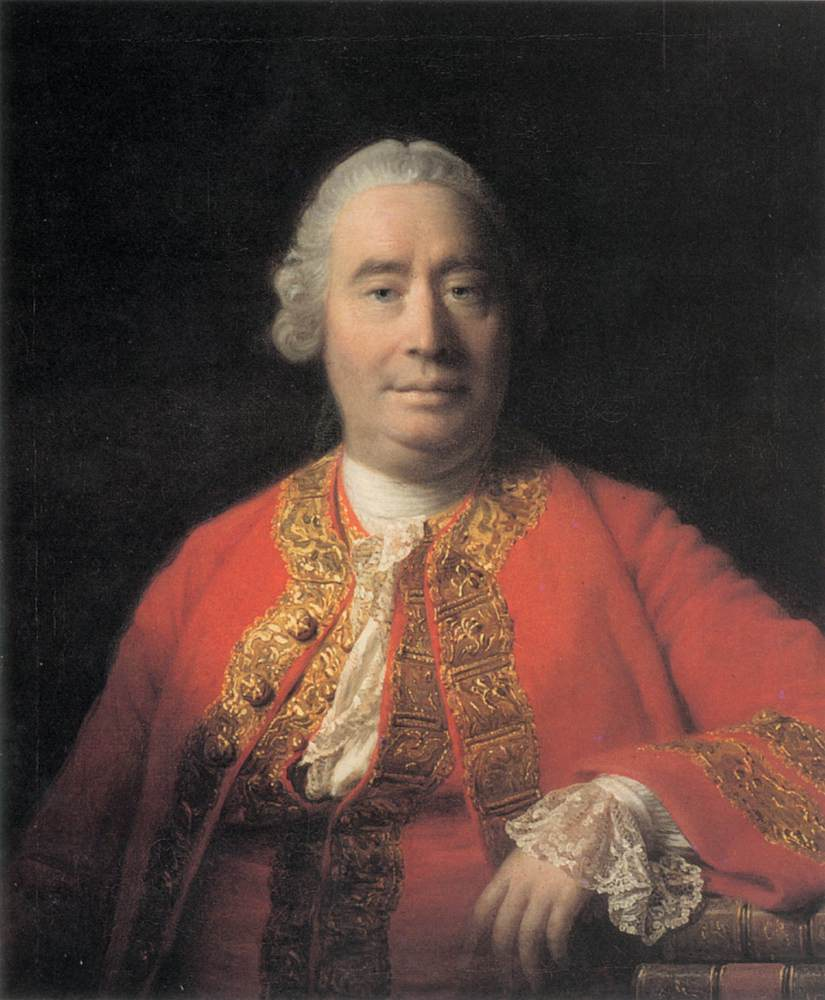
\includegraphics[height=4cm]{../../../graphics/hume.jpg}
            \end{column}
            \begin{column}{7cm}
                \begin{itemize}
                    \item The \alert{genealogy} of justice
                    \item The \alert{moral beauty} of just acts
                \end{itemize}
            \end{column}
        \end{columns}
}

% section hume_s_positive_account (end)

\section{The Genealogy of Justice}\label{sec:the_genealogy_of_justice} % (fold)

So far we have observed that the natural and artificial virtues differ in the following two respects:

\begin{itemize}
    \item Whereas the natural virtues are implanted instincts, the artificial virtues are not. The artificial virtues, instead of being dispositions native to human beings, are dispositions to behave in accordance with a general scheme or convention, itself the product of human artifice.
    \item Whereas the manifestation of the natural virtues invariably results in good, the manifestation of the artificial virtues does not invariably result in good---not every observance of the general scheme or convention benefits either the private individual or the public. It is the general compliance with the scheme or convention that benefits the public and not any particular observance of that general scheme.
\end{itemize}

A third difference is presently relevant:

\begin{itemize}
    \item Whereas the natural virtues are partial and unequal, the artificial virtues are impartial and equal.
\end{itemize}

% \textbf{See Figure~\ref{fig:slide2}.}
% 
% \begin{figure}[ht]
%     \begin{center}
%         \includeslide[height=5cm]{slide2<3>}
%     \end{center}
%     \caption{The Partiality of Natural Virtue}
%     \label{fig:slide2}
% \end{figure}

\frame<presentation>[label=slide2]{
    \frametitle{The Partiality of Natural Virtue}
        \begin{columns}
            \begin{column}{3cm}
                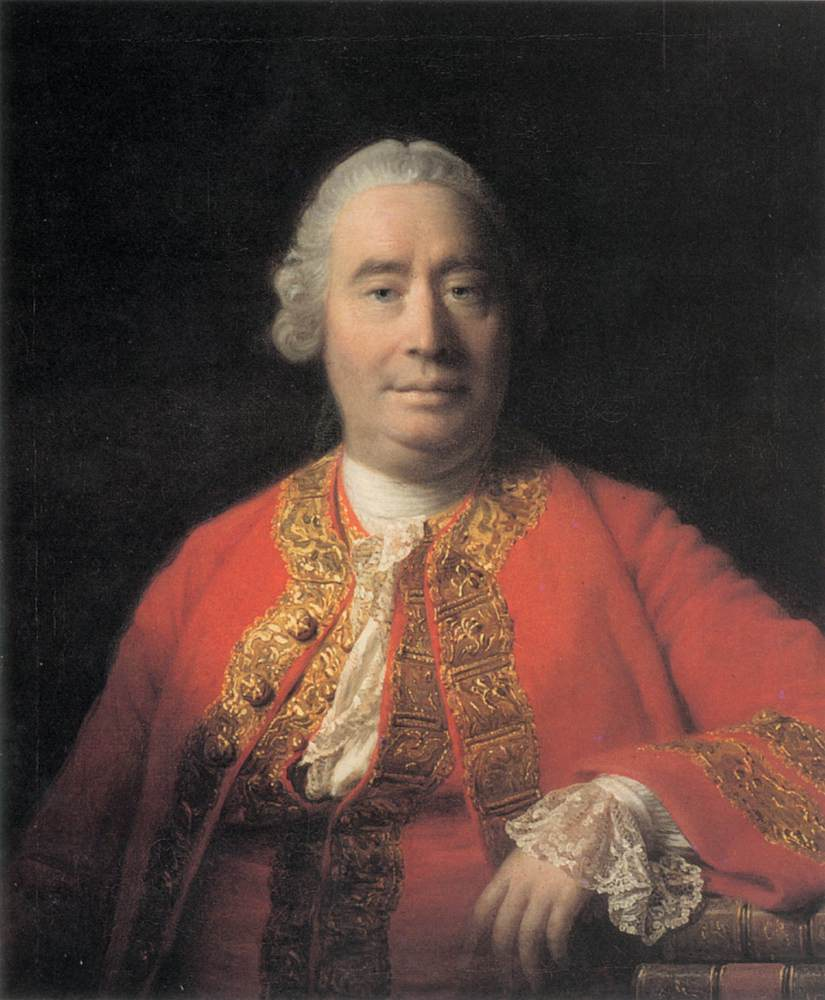
\includegraphics[height=4cm]{../../../graphics/hume.jpg}
            \end{column}
            \begin{column}{7cm}
                \begin{itemize}
                    \item<1-> Whereas the natural virtues are \alert{implanted instincts}, the artifical virtues are not. 
                    \item<2-> Whereas the manifestation of the natural virtues \alert{invariably results in good}, not so the manifestations of artificial virtue.
                    \item<3-> Whereas the natural virtues are \alert{partial and unequal}, the artificial virtues are \alert{impartial and equal}.
                \end{itemize}
            \end{column}
        \end{columns}
}

According to Hume, human beings are by nature partial, but this does not mean that every natural affection is selfish.

Hume's view is usefully contrasted with the \emph{Hobbist}. (The Hobbist is a creature of the philosophical bestiary not to be confused with the historical Hobbes. While there are superficial similarities, Hobbism is arguably the product of a historically salient misinterpretation of Hobbes.) According to the Hobbist, human beings are rational egoists:

\begin{description}
    \item[Rational Egoism] Human beings only ever act out of rational self-interest.
\end{description}

According to the Hobbist, all motivation is ultimately explained in terms of what benefits the individual. While we may appear to act for the sake of others, we only act in these ways because of the individual benefit it affords us, however indirectly. All apparently non-selfish motivation is merely apparent.

This is not at all Hume's conception of human motivation. Hume recognizes that human beings can act out of rational self-interest, that humans can be selfish and are, at times, inclined by the natural passion of avarice. However, Hume explicitly denies that we only ever act out of rational self-interest. Importantly, we are naturally inclined to act for the sake of others. Human beings are naturally benevolent, at least to some degree; just as they are naturally amiable to children. Human beings may be no angels, they may be selfish, but they have a natural concern for others.

What is important for Hume is not that human beings are \emph{selfish}---they are, though not exclusively so. Rather, what is important to Hume is that human beings are \emph{partial}. Consider our natural concern for others. Such concern is principally directed to those who we are related in important ways, by the bounds of kinship or friendship, say. While principally directed towards others who are contiguous or similar, a concern for others can be extended to those who are distant and unknown to us through the operations of imagination and sympathy. However, because of the natural association of ideas, our concern for the distant and and unknown is considerably weaker than our concern for our kin. Our natural affection for others may refute the Hobbist contention that we only ever act selfishly, but our natural concern for others is not impartial---we do not have equal concern for all. We are naturally more concerned for those who are importantly related to us in some way, who are affiliated with us in some way, who are proper to us. We are naturally less concerned, if at all, for the distant and unkown. While we may not be exclusively selfish, our natural concern for others is partial and unequal.

% \textbf{See Figure~\ref{fig:slide3}.}
% 
% \begin{figure}[ht]
%     \begin{center}
%         \includeslide[height=5cm]{slide3<1>}
%     \end{center}
%     \caption{Caption}
%     \label{fig:slide3}
% \end{figure}

\frame<presentation>[label=slide3]{
    \frametitle{\emph{Partial}, Not \emph{Selfish}}
        \begin{columns}
            \begin{column}{3cm}
                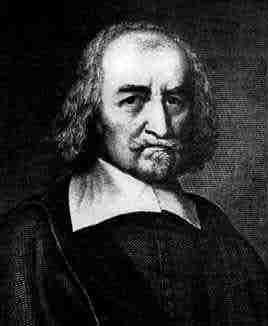
\includegraphics[height=4cm]{../../../graphics/hobbes.jpg}
            \end{column}
            \begin{column}{7cm}
                \begin{itemize}
                    \item \alert{Rational Egoism}: Human beings only ever act out of rational self-interest
                    \item The Hobbist, but note Hume is a rational egoist. According to Hume, the natural affections are, instead, \emph{partial}
                \end{itemize}
            \end{column}
        \end{columns}
}

According to Hume, the conventions of justice are only possible in certain circumstances. Call these \emph{the circumstances of justice}. The circumstanes of justice divide into two kinds, there are objective and subjective circumstances:

\begin{itemize}
    \item \textbf{Objective circumstances of justice}:
        \begin{enumerate}
            \item \emph{The scanty provision of nature}---while human beings have needs, there exists in nature a scarcity of objects that meet our needs.
            \item \emph{The easy exchange of objects}---at least some of the objects of need are easily exchangeable between individuals
        \end{enumerate}
    \item \textbf{Subjective circumstances of justice}:
        \begin{enumerate}
            \item \emph{Selfishness}---as human beings we are naturally, if not exclusively, inclined to act on our own interests. While we have a natural concern for others, self-interest remains for Hume a powerful source of human motivation.
            \item \emph{Benevolence}---as human beings we have a natural concern for the well being of others, at least those who are affiliated with us in a certain way.
        \end{enumerate}
\end{itemize}

While in the \emph{Treatise} Hume speaks of \emph{confined generosity}, in the \emph{Second Enquiry} Hume speaks of \emph{benevolence}. I follow the terminology of the \emph{Second Enquiry} since talk of confined generosity can mislead. If the emphasis is placed on ``confined'' then ``confined generosity'' can be read as a wry description of human selfishness. If the emphasis is instead placed on ``generosity'' then the qualification ``confined'' can be read as registering the partial nature of our benevolent concern for others. This latter interpretation is at least consistent with doctrine of the \emph{Second Enquiry}.

Justice, understood narrowly as a general scheme or convention governing property, is only possible if each of the circumstances of justice obtain. If any one of them fail, then it would not be possible to establish conventions of justice in those circumstances.

% \textbf{See Figure~\ref{fig:slide4}.}
% 
% \begin{figure}[ht]
%     \begin{center}
%         \includeslide[height=5cm]{slide4<1>}
%     \end{center}
%     \caption{The Circumstances of Justice}
%     \label{fig:slide4}
% \end{figure}

\frame<presentation>[label=slide4]{
    \frametitle{The Circumstances of Justice}
        \begin{columns}
            \begin{column}{3cm}
                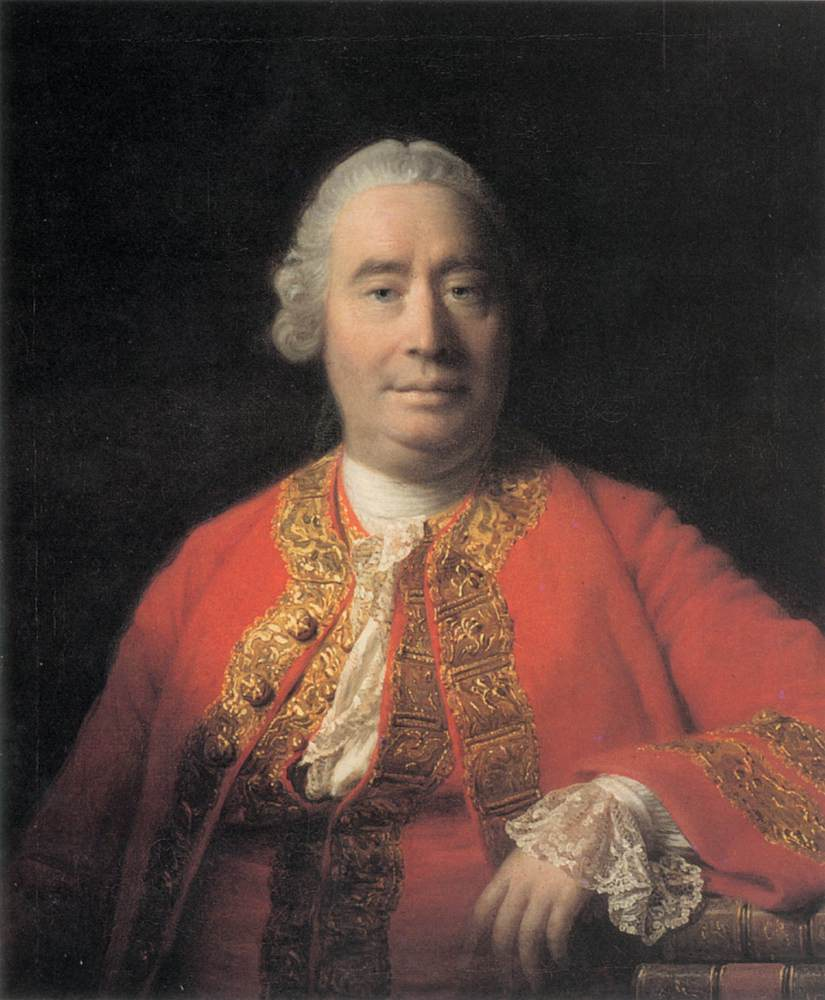
\includegraphics[height=4cm]{../../../graphics/hume.jpg}
            \end{column}
            \begin{column}{7cm}
                \begin{itemize}
                    \item \alert{Objective} circumstances of justice
                        \begin{itemize}
                            \item The scanty provision of nature
                            \item The easy exchange of goods
                        \end{itemize}
                    \item \alert{Subjective} circumstances of justice
                        \begin{itemize}
                            \item Selfishness
                            \item Confined benevolence
                        \end{itemize}
                \end{itemize}
            \end{column}
        \end{columns}
}

To illustrate this Hume invites us to consider two thought experiments:

\begin{enumerate}
	\item The State of Nature
	\item The Golden Age
\end{enumerate}

\emph{The State of Nature} is the state of humankind prior to the establishment of society. Hume doubts that humans were ever in the state of nature, or if there were, he doubts whether they remained in that rude and natural state for very long. He thus rejects as implausible the Hobbist description of it as ``the war of all against all''. (Indeed, like Rousseau, he seems to think that society, and not the lack of it, is more likely to engender conflict.) However, Hume does concede that in cases of extremity where the needs of humanity vastly outweigh the bounty of nature such that not all could survive, a natural concern for self-preservation could not be reasonably constrained by the needs of others. In such circumstances, there would be no motivation to observe general rules governing property, and the conventions of justice could neither be established nor sustained in circumstances of extreme want.

\emph{The Golden Age} is, according to to the poets, ``the most charming and most peaceable condition, that can possibly be imagin'd'':

\begin{quote}
	The seasons, in that first age of nature, were so temperate, if we may believe the poets, that there was no necessity for men to provide themselves with cloaths and houses as a security against the violence of heat and cold. The rivers flow'd with wine and milk: The oaks yielded honey; and nature spontaneously produc'd her greatest delicacies. Nor were these the chief advantages of that happy age. The storms and tempests were not alone remov'd from nature; but those more furious tempests were unknown to human breasts, which now cause such uproar, and engender such confusion. Avarice, ambition, cruelty, selfishness, were never heard of: Cordial affection, compassion, sympathy, were the only movements, with which the human mind was yet acquainted. Even the distinction of mine and thine was banish'd from that happy race of mortals, and carry'd with them the very notions of property and obligation, justice and injustice.
\end{quote}

The poets, in envisioning the golden age, imagine the bounty of nature to increase so that there is no want, and the benevolence of humanity to increase so that there is no avarice or jealousy. Since establishing general rules of property would lack utility in the golden age---there is no inconvenience to be remedied by establishing the conventions of justice---such conventions would never be established. Justice would simply not be possible in the Golden Age

What unites these various thought experiments is that, in each, at least one of the circumstances of justice is imagined not to obtain with the consequence that it is inconceivable the conventions of justice could be established in the imagined state of affairs. In cirumstances of extremity, if not the state of nature as the Hobbist conceives of it, there is scarcity, benevolence is not in operation, and justice is not possible. In the Golden Age, there is abundance, selfish inclinations is not in operation, and again justice is not possible.

% \textbf{See Figure~\ref{fig:slide5}.}
% 
% \begin{figure}[ht]
%     \begin{center}
%         \includeslide[height=5cm]{slide5<1>}
%     \end{center}
%     \caption{Two Thought Experiments}
%     \label{fig:slide5}
% \end{figure}

\frame<presentation>[label=slide5]{
    \frametitle{Two Thought Experiments}
        \begin{columns}
            \begin{column}{3cm}
                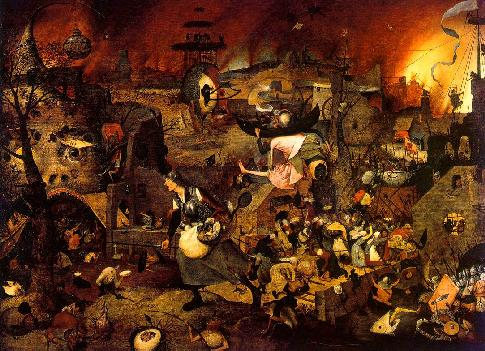
\includegraphics[width=3cm]{../../graphics/state_of_nature.jpg}\\
                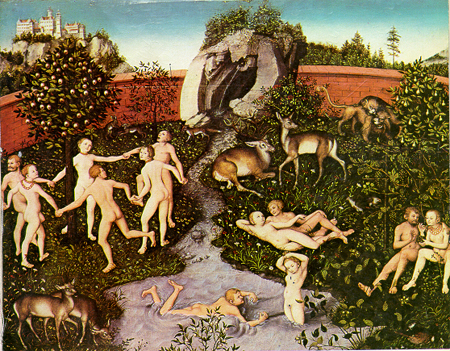
\includegraphics[width=3cm]{../../../graphics/golden_age.jpg}
            \end{column}
            \begin{column}{7cm}
                \begin{enumerate}
                    \item \alert{The State of Nature}
                    \item \alert{The Golden Age}
                \end{enumerate}
            \end{column}
        \end{columns}
}

What is the problem that convention is meant to solve?

Hume, like the Hobbist, maintains, that the rules of justice are indispensable for society. Given the evident disadvantages of life outside the society, human beings have an interest in the establishment of society. The Hobbist sees this as posing related coordinative and motivitional problems. The coordinative problem is how we can come to recognize the need to regulate our behavior for mutual advantage in this way. The motivational problem is how we can be moved by this concern in the face of more immediate, and potentially more attractive, individual concerns.

Crucially, however, these are not Hume's problems. Hume' problem is not how, on purely self-interested grounds, human beings can be moved to constrain at least some of their ends for the sake of mutual advantage. Conventions of justice---specifically, general rules governing property---could not be a solution that could be proposed and acted upon by human beings in the rude and natural state:

\begin{quote}
	The idea of justice can never serve to this purpose, or be taken for a natural principle, capable of inspiring men with an equitable conduct towards each other. That virtue, as it is now understood, wou'd never have been dream'd of among rude and savage men. (\emph{Treatise}, 3.2.2)
\end{quote}

Conventions of justice could not be the solution to the coordination and motivational problems because of a more fundamental problem about our idea of justice. Hume seems to think that human beings in the rude and natural state lack the very idea of justice, and so could not propose the establishment of the conventions of justice as a remedy to the disadvantages of life outside of society.

Questions about the origins of our ideas are familiar from Book I of the \emph{Treatise} where Hume posed probing questions about the origins of metaphysically important ideas such as causation and the self. Moreover, given the first principle of the science of human nature, questions about the origin of our ideas tend to follow a certain pattern---ideas are copies of impressions, and so an adequate account of their origin involves explaining how these ideas are the products of impressions that they resemble. Moreover, it can seem that this pattern is continued in Book III. According to Hume's sentimentalism, all moral distinctions are grounded in sentiment, a kind of impression. So to ask for the idea of justice is to ask for the impression upon which the distinction between justice and injustice is grounded. However, the distinction cannot be grounded in any natural human motivation. The circle provided one obstacle. Here, however, Hume emphasizes another, the partiality of natural affection:

\begin{quote}
	Now it appears, that in the original frame of our mind, our strongest attention is confin'd to ourselves; our next is extended to our relations and acquaintance; and 'tis only the weakest which reaches to strangers and indifferent persons. This partiality, then, and unequal affection, must not only have an influence on our behaviour and conduct in society, but even on our ideas of vice and virtue. (\emph{Treatise}, 3.2.2)
\end{quote}

Evidently the idea of justice must be impartial and equal in the way that none of our natural passions are. Since our natural passions are partial and unequal, they cannot give rise to the idea of justice since it resembles no natural passion in being impartial and equal.

% \textbf{See Figure~\ref{fig:slide6}.}
% 
% \begin{figure}[ht]
%     \begin{center}
%         \includeslide[height=5cm]{slide6<2>}
%     \end{center}
%     \caption{The Problem}
%     \label{fig:slide6}
% \end{figure}

\frame<presentation>[label=slide6]{
    \frametitle{The Problem}
        \begin{columns}
            \begin{column}{3cm}
                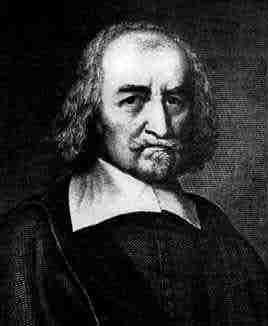
\includegraphics[width=3cm]{../../../graphics/hobbes.jpg}\\
                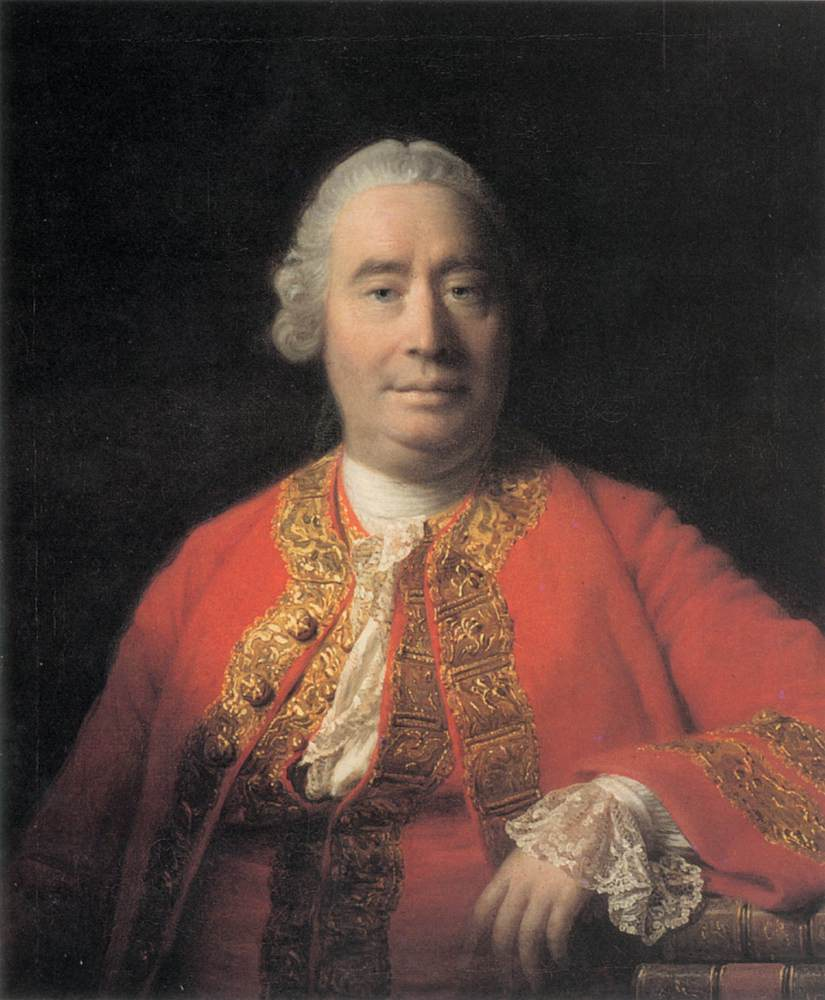
\includegraphics[width=3cm]{../../../graphics/hume.jpg}
            \end{column}
            \begin{column}{7cm}
                \begin{itemize}
                    \item<1-> For the \emph{Hobbist}, the problem concerns \alert{coordination} and \alert{motivation}
                    \item<2-> For \emph{Hume}, the problem concerns \alert{the origin of the idea of justice}
                \end{itemize}
            \end{column}
        \end{columns}
}

Conventions play a role in establishing our idea of justice since by means of them human beings restrain the ``partial and contradictory motions'' of their natural affections.

Hume makes negative and positive claims about conventions---he first tells us what they are not and then tells us about the attitudes that give rise to the conventions:

\begin{enumerate}
	\item \emph{Conventions are not promises}: Promises themselves are based on human conventions and so cannot give rise to them. This is Hume's central anti-contractarian point, his targets are the Hobbist and Rousseau.
	\item \emph{Conventions involve a general sense of common interest}: This is Hume's gloss on the attitudes involved in entering into a convention.
\end{enumerate}

Hume's negative claim is only substantiated in a later chapter dedicated to the nature of promising where he explains how conventions make promising possible. If the suitable conventions are among the conditions that make conventions possible, then promises cannot themselves give rise to conventions. Hume's case of the oarsmen is supposed to provide intuitive support for this claim.

Hume's positive characterization of the attitudes that give rise to convention requires some interpretation to unpack. Fortunately, Hume explains further:

\begin{quote}
	I observe, that it will be for my interest to leave another in the possession of his goods, provided he will act in the same manner with regard to me. He is sensible of a like interest in the regulation of his conduct. When this common sense of interest is mutually express'd, and is known to both, it produces a suitable resolution and behaviour. And this may properly enough be call'd a convention or agreement betwixt us, tho' without the interposition of a promise; since the actions of each of us have a reference to those of the other, and are perform'd upon the supposition, that something is to be perform'd on the other part.
\end{quote}

How are we to understand this ``sutiable resolution''? The resolution can be understood as an intention or commitment (as when we \emph{resolve} to undertake some course of conduct) that the conflicting parties settle upon when their common interest is mutually expressed and known to both. Specifically, the suitable resolution is a conditional intention to leave the other in possession his goods provided he does the same. Notice that this intention is framed purely from self interest. It thus does not depend on the relations one bears to the conflicting part in the way that love or confined benevolence does. The relevant feature of the conflicting party is not that similarity or affiliation to us, but their acceptance of the conditional commitment that one has undertaken. The suitable resolution is thus impartial and equal in the way that our natural affections are not and thus is an impression that can give rise to the idea of justice.

To sum up: Justice only arises under certain conditions. The circumstances of justice include the scanty provision of nature and man's selfishness and confined benevolence. The natural affections of human beings are partial and have a tendency to conflict. In such circumstances it is is in the self interest of each to constrain at least some of their ends for the sake of mutual advantage. Specifically, it is in the interest of each to leave the other in possession of their goods provided that they do the same. When this general sense of common interest is mutually expressed and known to both, this gives rise to the corresponding conditional commitment. This commitment, since it only requires the cocommitment of the conflicting party, does not depend upon their affiliation or any other relevant relation to us. It is thus impartial and equal in a manner suitable to give rise to the idea of justice.

% \textbf{See Figure~\ref{fig:slide7}.}
% 
% \begin{figure}[ht]
%     \begin{center}
%         \includeslide[height=5cm]{slide7<1>}
%     \end{center}
%     \caption{Convention}
%     \label{fig:slide7}
% \end{figure}

\frame<presentation>[label=slide7]{
    \frametitle{Convention}
        \begin{columns}
            \begin{column}{3cm}
                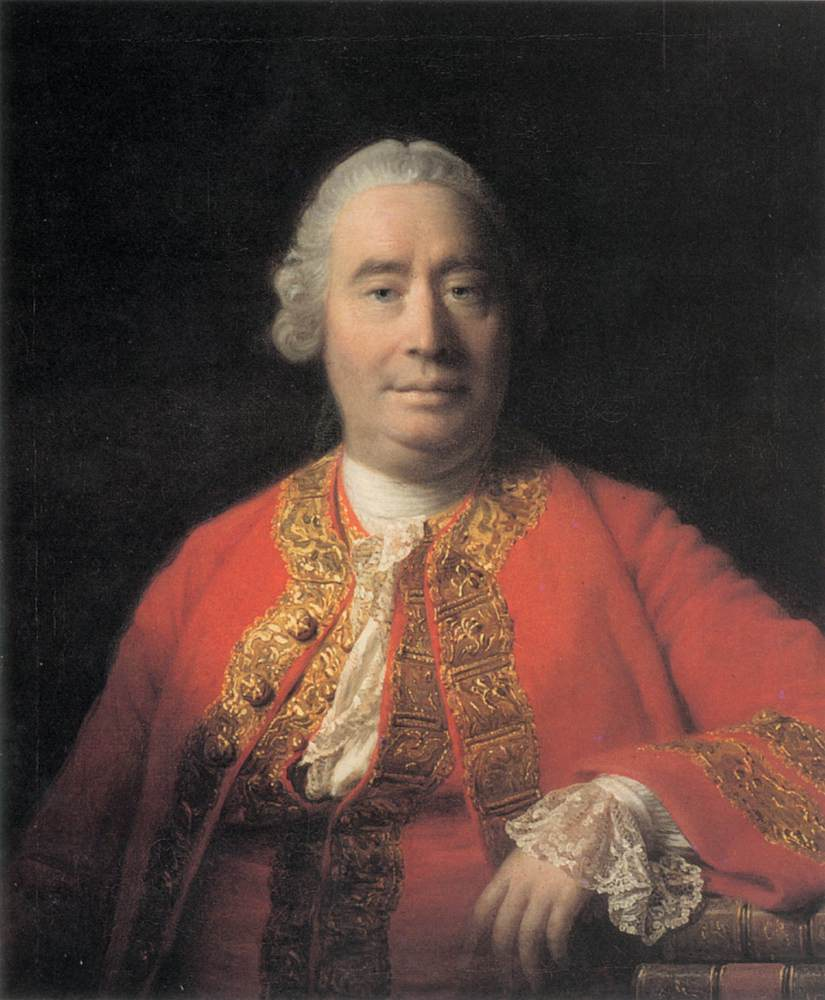
\includegraphics[height=4cm]{../../../graphics/hume.jpg}
            \end{column}
            \begin{column}{7cm}
                \begin{itemize}
                    \item Conventions are not promises
                    \item Convetions involve a general sense of common interest
                \end{itemize}
            \end{column}
        \end{columns}
}

% section the_genealogy_of_justice (end)

\section{The Moral Beauty of Justice}\label{sec:the_moral_beauty_of_justice} % (fold)

% TODO: This needs to be rewritten to bring in sympathy

The common sense of interest and the suitable resolution that it gives rise to may be the original motive to justice, but it does not explain the merit that attaches to particular observances of the rules of justice nor why these are the obejcts of moral approbation. While Hume has provided a genealogy of justice, he has yet to account for the moral beauty of its observances. He has yet to explain why we annex the idea of virtue to justice and vice to injustice.

The suitable resolution grounded in the common sense of interest may be sufficient motivation to observe the the conventions of justice. However, when society stabilizes and expands it has a tendency to wane:

\begin{quote}
	But when society has become numerous, and has encreas'd to a tribe or nation, this interest is more remote; nor do men so readily perceive, that disorder and confusion follow upon every breach of these rules, as in a more narrow and contracted society.
\end{quote}

Fortunately, there arises in human beings in a civilized state a subsidiary motivation:

\begin{quote}
	But tho' in our own actions we may frequently lose sight of that interest, which we have in maintaining order, and may follow a lesser and more present interest, we never fail to observe the prejudice we receive, either mediately or immediately, from the injustice of others; as not being in that case either blinded by passion, or byass'd by any contrary temptation. Nay when the injustice is so distant from us, as no way to affect our interest, it still displeases us; because we consider it as prejudicial to human society, and pernicious to every one that approaches the person guilty of it.
\end{quote}

Recall the sentimentalist conception of virtue that Hume describes in chapter one. Virtue consists in those actions, passions, and characters that give rise to pleasure upon the general view or survey, and vice consists in those actions, passions, and characters that give rise to displeasure upon the general view or survey. In a civilized state, human beings have a tendency to be displeased by acts of injustice even when neither they nor their kith and kin are the victims of this justice. Since this displeasure is impartial in this way, it can only be the determination of vice in the act of injustice. Hume suggests that it is the operation of sympathy that underlies this sense of duty but does not elaborate, promising to return to this when discussing the natural virtues.

In a civilized state, we are encouraged to take pleasure in acts of justice and displeasure in acts of injustice by a variety of factors, including public praise and blame (such as the exhortations of politicians), private education (as afforded to us by our parents), and a natural concern for our reputation. For a persion raised in a civilized state, these various factors encourage them to develop a sensibility that attaches a moral beauty to particular observances of the general scheme or convention. This value we attach to particular observances of the convention affords us an additional motivation to act justly.

We have seen how Hume sought to accommodate the vulgar’s talk of the combat of reason and passion, despite reason’s impotence, by reconstruing it as the combat between the calm and violent passions. We can see in Hume’s account of the artificial virtue of justice an attempt to accommodate another phenomena of morality recognized by the vulgar—the potential conflict of duty and inclination (about which Kant will have much to say). Just as talk of combat of reason and the passions seemed to threaten Hume’s contention that reason is and ought only to be the slave of the passions, so to talk of the conflict of duty and inclination seems to threaten Hume’s sentimentalist account.

Recall that the manifestation of a natural virtue invariably results in some good, but that this fails of the artifical virtue of justice. A particualr observance of the conventions of justice may result in personal or public harm. Public utility attaches to the general scheme or convention and not to any particular observance. So there may not be anything that recommends a particular observance of the conventions of justice from a partial point of view. Self interest may prompt the suitable resolution that institutes the rules of justice, but when moral beauty is attached to particular observances, there arises an additional motivation. In developing a sense of duty, we are motivated to act in accordance with the rules of justice just because that is what justice demands of us regardless of whether or not there is anything else in that act that would recommend itself to us. Since conformity to convention does not require that the particular observance have a single attractive feature, it may lack an attractive feature and may in fact be unpleasant.

Hume’s account of the artificial virtues allows him to accommodate the conflict of duty and inclination within a sentimentalist framework.

% \textbf{See Figure~\ref{fig:slide8}.}
% 
% \begin{figure}[ht]
%     \begin{center}
%         \includeslide[height=5cm]{slide8<2>}
%     \end{center}
%     \caption{The Moral Beauty of Justice}
%     \label{fig:slide8}
% \end{figure}

\frame<presentation>[label=slide8]{
    \frametitle{The Moral Beauty of Justice}
        \begin{columns}
            \begin{column}{3cm}
                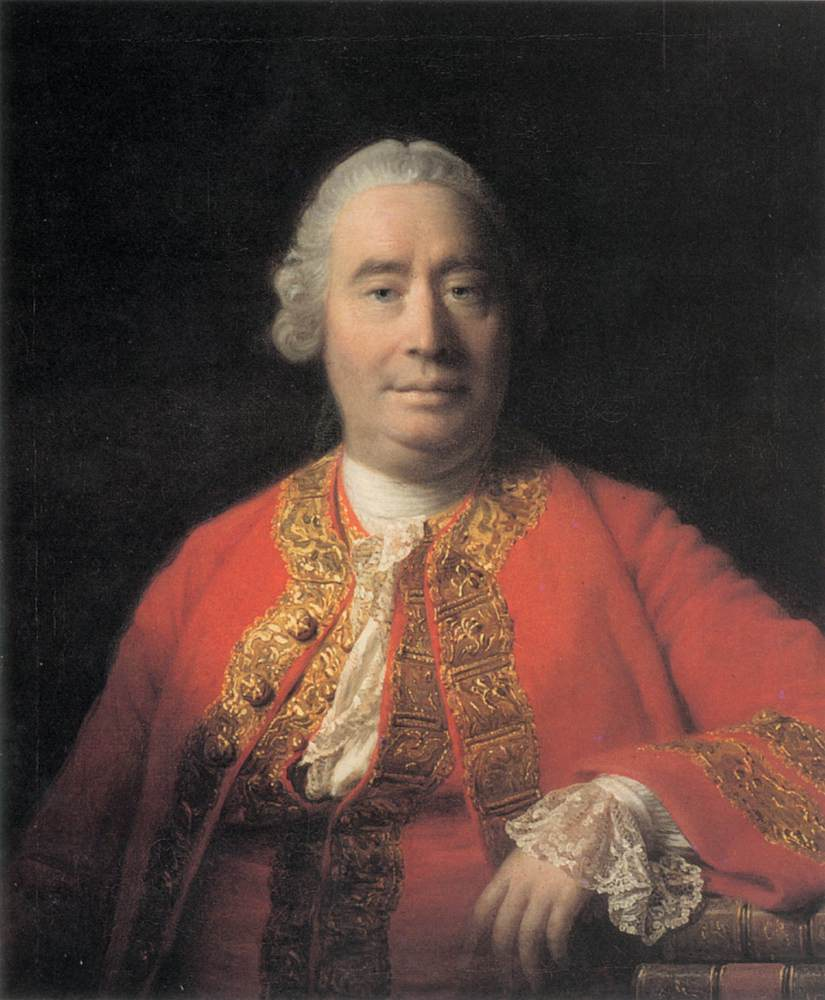
\includegraphics[height=4cm]{../../../graphics/hume.jpg}
            \end{column}
            \begin{column}{7cm}
                \begin{itemize}
                    \item<1-> Provides additional motivation to act justly
                    \item<2-> Allows for a sentimentalist accommodation of the conflict of duty \& inclination
                \end{itemize}
            \end{column}
        \end{columns}
}

% section the_moral_beauty_of_justice (end)

\section{The Circle Revisited}\label{sec:the_circle_revisited} % (fold)

Let's pause to consider how Hume's positive account of justice as an artificial virtue coheres with his negative argument that justice is not a natural virtue.

Recall, Hume argues that justice is not a natural virtue since the contrary supposition involves a vicious circularity:
\begin{quote}
    From all this it follows, that we naturally have no real or universal motive for observing the laws of equity, but the very equity and merit of that observance; and as no action can be equitable or meritorious, where it cannot arise form some separate motive, there is here an evident sophistry and reasoning in a circle. Unless, therefore, we will allow, that nature has establish’d a sophistry, and render’d it necessary and unavoidable, we must allow, that the sense of justice and injustice is not deriv’d from nature, but arises artificially, tho’ necessarily from education, and human conventions. (\emph{Treatise}, 3.2.1.17)
\end{quote}

Recall that with respect to the natural virtues, the motive to virtuous action is what bestows merit upon that action. Consider kindness to children. When you feed a hungry child, the motive is kindness, and it is the amiableness of this action, its being motivated by kindness, that bestows merit upon the action and makes it the object of moral approbation. So: 
\begin{enumerate}
    \item naturally virtuous actions have merit and are the object of moral approbation insofar as they are motivated in the relevant way, and 
    \item it is their being so motivated that bestows merit upon them and makes them the object of approbation.
\end{enumerate}

If justice were a natural virtue, then, (1) just actions would have merit and be the object of moral approbation insofar as they are motivated in the relevant way, and (2) it is their being so motivated that would bestow merit upon them and make them the object of approbation. However, just actions do not satisfy these two conditions---Hume's circle established that. What could the relevant motive be? While a regard to the justice of the action can motivate a person in a civilized state to act justly, it could not bestow merit upon that action. Moreover, no independently specified natural motive, such as self-love and public and private benevolence, could be the motive to just action. Since justice does not satisfy these two conditions, justice could not be a natural virtue.

On Hume's genealogical account of justice, the first motive to justice, the resolution prompted by a general sense of common interest mutually expressed may establish the conventions of justice, but a \emph{distinct} motive bestows merit upon them. It is not the resolution prompted by a general sense of common interest that bestows merit upon a just act, but, rather, sympathy with the public utitlity of the general scheme or convention that bestows merit upon its observance. There is no single motive that plays both roles. This is how justice, properly conceived, avoids the circularity---it is only by conceiving of justice as an artificial virtue that we can avoid ``evident sophistry and reasoning in a circle''.


% section the_circle_revisited (end)

\section{Self-Vindication}\label{sec:self_vindication} % (fold)

When we bagan, I emphasized that Hume's project is primarily \emph{descriptive} and \emph{explanatory} as opposed to \emph{prescriptive} and \emph{justificatory}. However, while Hume's sentimentalism purports to explain the moral judgments that we make, given the character of that explanation, it also justifies or vindicates these moral judgments.

Hume believes that once we understand fully the sentimentalist explanation of moral judgments, we will naturally approve of, not only these judgments, but also of our sense of morals and the principles that give rise to it:

\begin{quote}
	All lovers of virtue (and such we all are in speculation, however we may degenerate in practice) must certainly be pleas'd to see moral distinctions deriv'd from so noble a source, which gives us a just notion both of the generosity and capacity of human nature. It requires but very little knowledge of human affairs to perceive, that a sense of morals is a principle inherent in the soul, and one of the most powerful that enters into the composition. But this sense must certainly acquire new force, when reflecting on itself, it approves of those principles, from whence it is deriv'd, and finds nothing but what is great and good in its rise and origin.
\end{quote}

This Hume sees as a distinct advantage of his sentimentalism, grounded as it is in the operation of human sympathy, over the sentimentalism of his predecessor, Francis Hutcheson:

\begin{quote}
	Those who resolve the sense of morals into original instincts of the human mind, may defend the cause of virtue with sufficient authority; but want the advantage, which those possess, who account for that sense by an extensive sympathy with mankind. According to their system, not only virtue must be approv'd of, but also the sense of virtue: And not only that sense, but also the principles, from whence it is deriv'd. So that nothing is presented on any side, but what is laudable and good.
\end{quote}

Notice for something to have merit and to be the object of moral approbation just is for that thing to give rise to a distinctive kind of pleasure upon the general view or survey. If not only our moral judgments, but our sense of morals and the principles that give rise to them would please a Judicious Spectator, then these have merit and are the proper objects of moral approbation. Hume's new science of human nature is primarily descriptive and explanatory in its ambitions, as opposed to prescriptive and justificatory. Moral science seeks to describe diverse phenomena of human psychology and activity and explain these in terms of a few general principles. Moral science does not seek to prescribe that we make certain moral judgments. He is not engaged in any casuistry, nor is he offering a moral sermon or panygeric to Virtue. He is not recommending moral judgments to his audience. hume takes it for granted that he agrees in large measure with the moral judgments of his audience. Nor does moral science seek to justify the moral judgments that we actually do make. Hume is not trying to \emph{justify} the moral judgments we make. He is not trying to persuade a moral skeptic. Nevertheless once the explanation is set up and understood, we naturally approve of these principles and so perceive nothing that is not laudable and good. Hume's sentimentalist explanation of morals purports to vindicate itself.

The knowledge that a Humean moral scientist seeks is a kind of self-knowledge. The moral scientist seeks to explain the distinctions we make between vice and virtue in terms of our common human nature extended, where it is, by human convention. In learning about the few general principles that govern the diverse phenomena of human sentiment and that determine our judgments of vice and virtue, we learn about ourselves. We learn what kind of creatures we are.

While reason alone can neither determine the will nor oppose the passion's determination of the will, the self-knowledge we gain from Hume's moral science is not entirely indifferent to us. We come to naturally approve of our moral judgments and the principles that give rise to them. The human affective sensibility must be so configured, that the kind of self-knowledge afforded us by Hume's science of human nature is naturally pleasing to us upon the general view or survey. Not only is this self-knowledge pleasing to the human sensibility, it helps to transform our moral character. In particular, this self-knowledge strengthens our virtuous character:

\begin{quote}
	But this sense [sense of morals] must certainly acquire new force, when reflecting on itself, it approves of those principles, from whence it is deriv'd, and finds nothing but what is great and good in its rise and origin.
\end{quote}

So in approving of the the principles that determines our moral sense, the moral sense acquires new force, it gains new strength. Strength is a matter of causal control. Thus the causal influence of our sense of moral would tend to increase once it reflects on and approves of the principles upon which it is founded. In the case of the artificial virtues, such as justice, this would be manifest in an increased ability of the sense of duty, the sense of the moral beauty of particular observances of the conventions of justice, to oppose other passions that might conflict with it, such as selfishness or even benevolence. The categorical nature of these demands would be strengthened.

Though Hume sets out to be an anatomist of morals rather than a painter of virtue, nevertheless, the kind of self-knowledge we gain from the science of human nature has a natural tendency to transform our moral character by strengthening the operation of our moral sense. In gaining this self-knowledge, our moral character is transformed. Like Socrates before him, Hume sees a connection between self-knowledge and human virtue.

The precise connection he sees is perhaps the finest expression of Humean optimism. Humean optimism is characterized by a realistic if cheerful appraisal of human nature. We are not utterly selfish, but neither are we angels. Even given this realistic and balanced conception of human motivation, Hume is pleased with what it gives rise to, the moral distinctions it makes and the principles that govern these. A fact that is, perhaps, echoed by the literary pleasure we take in the nature and character of the author of the \emph{Treatise}.

% \textbf{See Figure~\ref{fig:slide9}.}
% 
% \begin{figure}[ht]
%     \begin{center}
%         \includeslide[height=5cm]{slide9<1>}
%     \end{center}
%     \caption{The Self-Vindication of Sentimentalism}
%     \label{fig:slide9}
% \end{figure}

\frame<presentation>[label=slide9]{
    \frametitle{The Self-Vindication of Sentimentalism}
        \small{All lovers of virtue (and such we all are in speculation, however we may degenerate in practice) must certainly be pleas'd to see moral distinctions deriv'd from so noble a source, which gives us a just notion both of the generosity and capacity of human nature. It requires but very little knowledge of human affairs to perceive, that a sense of morals is a principle inherent in the soul, and one of the most powerful that enters into the composition. But this sense must certainly acquire new force, when reflecting on itself, it approves of those principles, from whence it is deriv'd, and finds nothing but what is great and good in its rise and origin.}
}

% section self_vindication (end)

\section*{Summary}

\end{document}
